\documentclass{sciposter}
\usepackage{preposter} %pacote com o preambulo.
\usepackage{wrapfig,times}
\usepackage{slashbox}
\usepackage{tikz}
\usetikzlibrary{arrows.meta,
                calc, chains,
                quotes,
                positioning,
                shapes.geometric}
\usetikzlibrary{shapes, arrows, calc, positioning}
\usepackage{multicol}
\usepackage{multirow}
\usepackage{booktabs}
\usepackage{bm}
\usepackage{float}
\usepackage{caption}  
\definecolor{mainCol}{rgb}{1,1,0.99}
%\definecolor{BoxCol}{rgb}{0.13,0.67,0.29} % verde
\definecolor{BoxCol}{rgb}{0.1,0.590,0.705} % azul
\definecolor{TextCol}{rgb}{1,1,1}
\definecolor{SectionCol}{rgb}{0,0.10,0.305}

\usepackage[T1]{fontenc}
%\usepackage{Times}

\newcommand{\Z}{\mathbb Z} 
\newcommand{\F}{\mathbb F} % sigma-algebra

%\newcommand{\tablesize}{\fontsize{9}{11}\selectfont} % tamanho tabela

\allowdisplaybreaks[4] % para evitar espaços entre fórmulas

\renewcommand{\titlesize}{\Huge}


%%comandos exclusivos deste poster.
%\hypersetup{pdfpagelayout=SinglePage} %abre a pagina em modo simples
\geometry{paperwidth=90cm,paperheight=125cm,centering,
    textwidth=80cm,textheight=120cm,left=1.2cm,top=1.0cm, right=6.2cm}
%********************************************************************
\begin{document}

%%titulo
\colorbox{BoxCol}{
  \begin{minipage}{\textwidth}
    \color{white}{
      \begin{center}
        \Huge{\textbf{\vspace{0.2cm} \\
        Um aplicativo em \textit{Shiny} para ajuste do modelo de regressão quantílica Chen
        \vspace{0.7cm} \\}}
      \end{center}
    }
  \end{minipage}
}
\title{}
\vspace{-0.2cm}
\author{%\hspace{3.5cm}
\textbf{Alisson Rosa Pereira$^1$ \& Laís Helen Loose$^2$} 
} %%<-- seu nome
\institute{%\hspace{3.5cm}
%\vspace{-0.4cm}
$^1$Graduando em Estatística, UFSM - \texttt{alirpereira887@gmail.com}\\
$^2$Departamento de Estatística, UFSM - \texttt{lais.loose@ufsm.br}}
\vspace{-0.2cm}

\rightlogo[0.8]{imgs/brasao_cores}
\leftlogo[0.8]{imgs/logo.png}
 %logotipo da ufsm

\maketitle 

\vspace{-2.9cm}
\setlength{\columnseprule}{1.5pt}

%Texto em 2 colunas
\section*{\tituloA{24º Simpósio Nacional de Probabilidade e Estatística}}
\begin{multicols*}{2}{

%Paragrafo.
\setlength{\parindent}{0.4em}

\section*{\tituloA{Introdu\c{c}\~ao}}
\vspace{0.2cm}

Na última década, novas distribuições foram propostas com o objetivo principal de fornecer modelos mais flexíveis que possibilitem melhores soluções quando aplicados a dados reais. Uma distribuição bastante flexível e pouco explorada na literatura é a distribuição Chen, a qual foi introduzida por \cite{chen2000new} no contexto de análise de sobrevivência a fim de possibilitar ajustes em dados com taxa de falha crescentes e em formato de banheira.
\vspace{0.2cm}

Os modelos de regressão mais conhecidos e  geralmente utilizados em ajustes a dados reais são baseados no pressuposto de normalidade. No entanto, esta suposição nem sempre é satisfeita na prática. Como consequência, tem crescido o interesse no desenvolvimento e análise de modelos não gaussianos. Apesar de uma ampla gama de novos modelos estarem sendo desenvolvidos nos últimos anos, a falta de ferramentas computacionais para ajuste desses modelos ainda é um limitador para o amplo uso de recentes propostas em áreas aplicadas

\vspace{0.2cm}

Assim, o presente trabalho tem como objetivo apresentar o modelo de regressão quantílico Chen e fornecer uma ferramenta \textit{web} para ajuste do modelo. Para o desenvolvimento do aplicativo \textit{web} utilizamos o pacote Shiny, disponível na linguagem R \cite{R}.


\vspace{-0.2cm}

\section*{\tituloA{O modelo de regressão
quantílico Chen: formulação, inferência e adequação do ajuste}}
\vspace{0.2cm}

Se $Y$ é uma variável aleatória com distribuição Chen, então sua função densidade de probabilidade é dada pela forma abaixo \cite{chen2000new}
\vspace*{-0.1cm}
\begin{align}
\label{densidade}
f(y;\lambda, \delta)= \delta\lambda y^{\lambda - 1} \exp \left\lbrace \delta \left[ 1-\exp(y^{\lambda})\right] +y^{\lambda} \right\rbrace  , \quad  y > 0,
\end{align}
em que $ \delta , \lambda > 0 $ são os parâmetros de forma.

Consideremos $\mu= Q(\tau;\lambda , \delta)$ e que $\delta$ possa ser escrito como $\delta=\dfrac{\log(1-\tau)}{1-\exp(\mu^{\lambda})}$. Reescrevendo a função densidade dada pela equação \eqref{densidade} em termos da expressão de $\delta$, a densidade reparametrizada em termos do quantil ($\mu$) fica dada por
\begin{align}
\label{rep}
f(y ; \lambda, \mu, \tau)= \dfrac{\log(1-\tau)}{1-\exp(\mu^{\lambda})} \lambda  y^{\lambda - 1} \exp \left[ \dfrac{\log(1-\tau)}{[1-\exp(\mu^{\lambda})]} \left[ 1-\exp(y^{\lambda}) \right] +y^{\lambda} \right]. 
\end{align}

%\vspace{-0.2cm}
%{\small

Dessa maneira podemos formalizar o modelo de regressão quantílico supondo $Y_1,\ldots, Y_n$  variáveis aleatórias independentes, em que cada $Y_t$, $t=1,\ldots,n$, segue a densidade em \eqref{rep} com quantil $\mu_t$, $\lambda$ um parâmetro desconhecido e $\tau \in (0,1)$ conhecido. Assumimos então que o quantil ($\mu_t$) de $y_t$  pode ser escrito como
\begin{align}\label{modelo}
g(\mu_t)=  \bm{x}_{t}^{\top} \bm{\beta}= \eta_t,
\end{align}
em que $\bm{\beta}= (\beta_0,\ldots, \beta_k)^{\top}$ é um vetor de parâmetros de regressão desconhecidos $( \bm{\beta} \in \mathbb{R}^{ k + 1}) $ e $\bm{x}_{t}^{\top}=(1, x_{t_1},\ldots, x_{t_k})$ são observações sobre $k$ covariáveis $(k<n)$,  que são assumidas como fixas e conhecidas. $\eta_t$ é chamado preditor linear, $g(\cdot)$ é uma função de ligação, monótona e duas vezes diferenciável, tal que $g: \mathbb{R}^{+}\rightarrow \mathbb{R}$. 

\vspace{0.2cm}
O modelo de regressão quantílico Chen é definido pelas expressões \eqref{rep} e \eqref{modelo} \cite{souza2021}. Devido a restrição de que $\mu_t > 0$, a função de ligação mais usual nesse contexto é a logarítmica, $g(\mu_t)=\log(\mu_t)$.

\vspace{0.2cm}

Seja $y_1, \ldots, y_n$ uma amostra do modelo de regressão quantílico Chen proposto e $\bm{\theta}=(\bm{\beta}^{\top}, \lambda)^{\top}$ o vetor de parâmetros. A função de log-verossimilhança baseada  nessa amostra  é dada por
\begin{align}\label{logvero}
\ell(\bm{\theta})=\sum\limits_{t=1}^{n}\log \{f(y_t; \lambda, \mu_t, \tau)\}.
\end{align}


Os estimadores de máxima verossimilhança do vetor paramétrico $\bm{\theta}= ( \bm{\beta}^{\top}, \lambda)^{\top}$ são obtidos pela maximização da log-verossimilhança. 



O vetor escore $\bm{U}(\bm{\theta})=(\bm{U}_{\bm{\beta}}(\bm{\theta})^\top , U_\lambda(\bm{\theta}))^\top $ é obtido pela diferenciação da função de log verossimilhança em relação a cada elemento de $\bm{\theta}$. Os vetores escore relativos a cada um dos parâmetros $\beta_i, i=1, \ldots, k+1$, do vetor da estrutura de regressão $\bm{\beta}$ e $\lambda$, são dados, respectivamente, por
\begin{align*}
& U_{\beta_i}(\bm{\theta})=\dfrac{\partial \ell(\bm{\theta})}{\partial\beta_i}= \sum\limits_{t=1}^{n}\frac{\partial \ell_t(\mu_t,\lambda)}{\partial\mu_t}\frac{d\mu_t}{d \eta_t}\frac{\partial\eta_t}{\partial\beta_i} \quad 
\mbox{ e } \quad U_\lambda(\bm{\bm{\theta}})=\frac{\partial \ell(\bm{\theta})}{\partial\lambda}= \sum\limits_{t=1}^{n}\frac{\partial \ell_t(\mu_t,\lambda)}{\partial\lambda}.
\end{align*}



Os estimadores de máxima verossimilhança $\widehat{\bm{\beta}}$ e $\widehat{\lambda}$ dos parâmetros  $\bm{\beta}$ e $\lambda$ são obtidos resolvendo o seguinte sistema de equações não lineares:
\begin{align}\label{system}
\left\{ \begin{array}{ll} \bm{U}_{\bm{\beta}}(\bm{\theta})&=\bm{0} ,\\
U_\lambda(\bm{\theta})&= 0 .\end{array} \right.
\end{align}

Este sistema  não possui solução analítica em forma fechada, sendo necessário o uso de algoritmos de otimização não lineares. No presente trabalho utilizamos o método de Nelder-Mead. 


%A matriz de informação observada é obtida tomando o negativo das segundas derivadas da função de log-verossimilhança $\ell(\bm{\theta})$, em  relação ao vetor de parâmetros, dada por

%\begin{align}\label{inf_fisher}
%\bm{J(\theta)} = - \dfrac{\partial^2 \ell(\bm{\theta})}{\partial\bm{\theta} %\partial\bm{\theta}^{\top}}.
%\end{align}
A matriz de informação esperada é dada por 
\begin{align*}
\bm{K}(\bm{\theta})=E\left[ - \dfrac{\partial^2 \ell(\bm{\theta})}{\partial\bm{\theta} \partial\bm{\theta}^{\top}}\right] = E[\bm{J}(\bm{\theta})].
\end{align*}
A distribuição Chen não tem expressões analíticas em forma fechada para os momentos, logo não é possível obter expressões analíticas para a matriz de informação de Fisher. A matriz de informação observada $\bm{J}(\widehat{\bm{\theta}})$ é um estimador consistente para $\bm{K}(\bm{\theta})$. Sendo assim, no presente trabalho utilizaremos a matriz de informação observada.

Sob condições usuais de regularidade, os estimadores de máxima verossimilhança  $\widehat{\bm{\theta}}$ de $\bm{\theta}$ são  consistentes, com distribuição aproximada normal $(k+2)$-variada, com vetor de médias $\bm{\theta}$ e matriz de variância e covariâncias  $\bm{K}(\bm{\theta})^{-1}$ em grandes amostras, ou seja,

\begin{equation*} \label{assint}
\left(\begin{array}{c} 
\widehat{\bm{\beta}} \\
\widehat{{\lambda}} \\
\end{array} \right ) \sim \mathcal{N}_{k+2}    \left( \left(\begin{array}{c} 
\bm{\beta} \\ 
\lambda \\
\end{array} \right ), \boldsymbol{K} (\boldsymbol{\theta})^{-1} \right ),
\end{equation*}
em que $\widehat{\bm{\beta}}$ e $\widehat{\lambda}$ são os estimadores de $\bm{\beta}$ e $\lambda$, respectivamente.
\vspace{0.2cm}

Para a avaliação do modelo utilizamos o coeficiente de determinação generalizado, definido por:
\begin{align}\label{r2}
R^2= 1 - \exp\left[ - \frac{2}{n} \left[ \ell(\widehat{\bm{\theta}}) -\ell(\widehat{\bm{\theta}}_0) \right] \right],
\end{align}
em que $\ell(\widehat{\bm{\theta}}_0)$ é a log verossimilhança maximizada do modelo sem regressores (nulo), $\ell(\widehat{\bm{\theta}})$  é a log verossimilhança maximizada do modelo ajustado e $n$ é o tamanho da amostra.

Ainda, para a avaliação do ajuste do modelo utilizamos o resíduo quantílico que é definido em \cite{dun1996} por:
\begin{align*}
 r_t= \Phi^{-1}\left\lbrace \int_{0}^{y_t}f(u_t; \widehat{\lambda}, \widehat{\mu}_t, \tau )du_t\right\rbrace,
\end{align*}
em que $\Phi(\cdot)$  é a função de distribuição acumulada da Normal padrão.
\vspace{0.2cm}

Dada a estrutura aqui citada elaboramos um aplicativo em Shiny que possibilita o ajuste e verificação dos pressupostos básicos do modelo. 
\vspace{-0.2cm}

\section*{\tituloA{Aplicativo Shiny - Estrutura}}
\vspace{0.2cm}

Para o ajuste do modelo em Shiny, são necessários alguns \textit{inputs} que devem ser fornecidos/escolhidos pelo usuário, sendo eles:

\begin{itemize}
  \item \textbf{Dados}: O usuário pode fazer \textit{upload} de um arquivo em formato {\tt csv}, ou então usar dados simulados.
  \item \textbf{Escolha da variável resposta ($Y$)}: O usuário pode selecionar a variável resposta dentre as variáveis disponíveis nos dados inicialmente fornecidos.
  \item \textbf{Seleção de covariáveis ($\bm{X}$):} As variáveis explicativas podem ser selecionadas usando a sintaxe de fórmulas disponível no R, ou seja, se deseja, por exemplo, usar as covariáveis $X_2$ e $X_3$ então usa-se {\tt X2 + X3}.
  \item \textbf{Escolha da função de ligação}: Pode-se escolher entre a função logarítmica (log) e raiz quadrada (sqrt).
  \item \textbf{Escolha do quantil}: A escolha do quantil pode ser feita escolhendo qualquer valor no intervalo (0,1) espaçado por 0.01.
\end{itemize}
Após a inserção de todos os \textit{inputs} necessários deve-se clicar em fit para que o modelo seja ajustado.




\vspace{0.4cm}


\begin{figure}
\centering
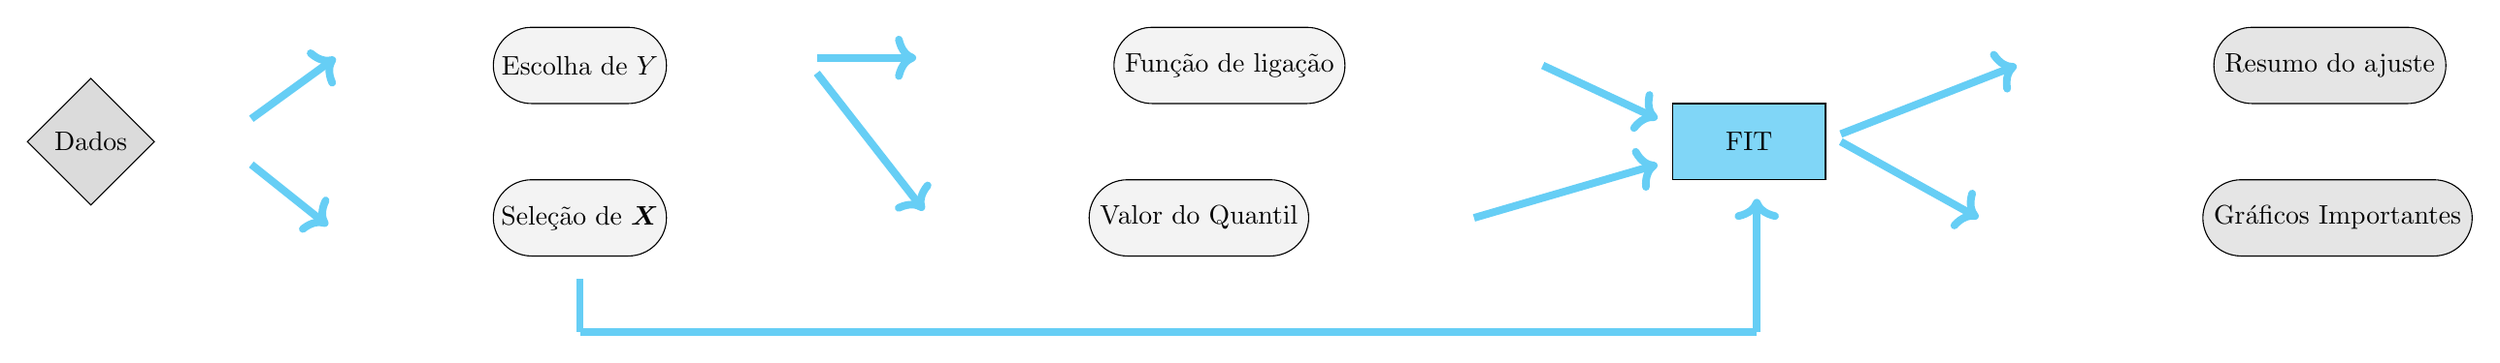
\begin{tikzpicture}
 
 
\node[diamond,draw, fill={rgb:black,1;white,6}] at (0,0) {Dados};


\draw[cyan!60, ->, line width=1mm] (2.1,0.3) -- (3.2,1.1);
\draw[cyan!60, ->, line width=1mm] (2.1,-0.3) -- (3.1,-1.1);

\node[draw,
    rounded rectangle, 
    minimum width=2.5cm,minimum height=1cm,  fill={rgb:black,0.5;white,10}] at (6.4,1){Escolha de $Y$};
\draw[cyan!60, ->, line width=1mm] (9.5,1.1) -- (10.8,1.1);
\draw[cyan!60, ->, line width=1mm, bend left] (9.5,0.9) -- (10.9,-0.9);


\node[draw,
    rounded rectangle, 
    minimum width=2.5cm,minimum height=1cm, fill={rgb:black,0.5;white,10}] at (6.4,-1){Seleção de $\bm{X}$};

\draw[cyan!60, -, line width=1mm, bend left] (6.4,-1.8) -- (6.4,-2.5);
\draw[cyan!60, -, line width=1mm] (6.4,-2.5) -- (21.8,-2.5);
\draw[cyan!60, ->, line width=1mm, bend left] (21.8,-2.5) -- (21.8,-0.75);

\node[draw,
    rounded rectangle, 
    minimum width=2.5cm,minimum height=1cm,  fill={rgb:black,0.5;white,10}] at (14.9,1){Função de ligação};
\draw[cyan!60, ->, line width=1mm] (19,1) -- (20.5,0.3);


\node[draw,
    rounded rectangle, 
    minimum width=2.5cm,minimum height=1cm,  fill={rgb:black,0.5;white,10}] at (14.5,-1){Valor do Quantil};
\draw[cyan!60, ->, line width=1mm] (18.1,-1) -- (20.5,-0.3);

\node[draw,
        fill=cyan!50,
        minimum width=2cm, 
        minimum height=1cm] at (21.7,0) {FIT};
\draw[cyan!60, ->, line width=1mm] (22.9,0.1) -- (25.2,1);
\draw[cyan!60, ->, line width=1mm] (22.9,0) -- (24.7,-1);


\node[draw,
    rounded rectangle, 
    minimum width=2.5cm,minimum height=1cm, fill={rgb:black,1;white,9}] at (29.3,1){Resumo do ajuste};
\node[draw,
    rounded rectangle, 
    minimum width=2.5cm,minimum height=1cm, fill={rgb:black,1;white,9}] at (29.4,-1){Gráficos Importantes};

 
	

\end{tikzpicture}

%\captionof{figure}{\textbf{ Fluxograma da Estrutura}}
\end{figure}

\vspace{0.5cm}

\centerline{Figura 1: \textbf{ Fluxograma da Estrutura}}







\section*{\tituloA{Resumo do Ajuste}}
\vspace{0.2cm}

Após o  modelo ser ajustado será fornecido um resumo do ajuste semelhante ao exemplo a seguir.


\vspace{0.2cm}

\begin{table}
\centering
\begin{tabular}{l| c | c | c | c}
\hline
\rowcolor{lightgray!40}
  & estimate & std\_error & z\_value & p\_value\\
\hline
lambda & 0.969 & 0.0162 & 59.9251 & <0.001\\
\hline
(Intercept) & -0.1632 & 0.0254 & 6.4333 & <0.001\\
\hline
V2 & 2.5776 & 0.0179 & 144.189 & <0.001\\
\hline
V3 & -2.0559 & 0.0156 & 131.487 & <0.001\\
\hline
V4 & 3.106 & 0.0218 & 142.7914 & <0.001\\
\hline
\end{tabular}
%\captionof{table}{Tabela Resumo}
\end{table}

\centerline{Tabela 1: \textbf{ Resumo do ajuste}}
\vspace{0.3cm}

A Tabela contém um resumo do ajuste incluindo as estimativas dos parâmetros, erro padrão e p-valores associados ao testes de hipóteses. Tem-se também algumas métricas de seleção de modelos, como AIC, BIC e RMSE, que são fornecidas no aplicativo.
\vspace{0.2cm}

São fornecidas outras quantidades de interesse, sendo elas:
\begin{itemize}
\item \textbf{Number of iteractions}: Indica a quantidade de iterações que foram necessárias para a convergência do método de otimização.
\item \textbf{Residuals}: Medidas descritivas básicas dos resíduos.
\item \textbf{R-squared}: Informa o valor do coeficiente de determinação generalizado, definido em \eqref{r2}

\vspace{0.2cm}

Uma tabela indicando medidas descritivas básicas sobre o banco de dados também é fornecida.
\end{itemize}

 


\section*{\tituloA{Gráficos Importantes}}
\vspace{0.2cm}

Os gráficos fornecidos para avaliar a qualidade do ajuste do modelo são:

\begin{itemize}
  \item \textbf{Resíduos vs Valores Preditos:} Útil para detecção de \textit{outliers}, em modelos bem ajustados os resíduos devem estar em torno de zero.
  \item \textbf{Densidade do Resíduo:} Espera-se que a densidade dos resíduos se comporte semelhante a uma normal padrão.
  \item \textbf{Resíduos vs Índices:} Se o modelo estiver bem ajustado os resíduos quantílicos possuem distribuição normal padrão, assim espera-se poucos valores fora do intervalo de -3 e 3.
  \item  \textbf{Envelope simulado:} Se a distribuição assumida é adequada, espera-se que os pontos se encontrem dentro das bandas de confiança.
\end{itemize}




\section*{\tituloA{Considerações finais}}
\vspace{0.2cm}
\begin{multicols}{2}{
\begin{itemize}
\item Atualmente está sendo desenvolvido um pacote em linguagem R para o uso do modelo de regressão quantílico Chen, onde pode-se ajustar o modelo e também avaliar a qualidade do ajuste.
Porém evidentemente tal abordagem necessita que o usuário
tenha conhecimentos básicos da linguagem R.
\item  O aplicativo em Shiny é uma boa alternativa para aqueles não tem ou não desejam ter conhecimento na linguagem R, mas desejam utilizar o modelo.
\end{itemize}


\begin{figure}[h]
\centering
\includegraphics[width=9cm]{imgs/frame.png}
\end{figure}
\centerline{\textbf{Acesse o Shiny aqui}}
%\tikzset{near start abs/.style={xshift=1cm}}
%\begin{tikzpicture}
%\node[inner sep=0pt] (shiny) at (10,1.5)
    %{\includegraphics[width=8cm]{frame.png}};
%\draw[cyan!60, -, line width=1.4mm] (2,-3) -- (5,-3);
%\draw[cyan!60, -, line width=1.4mm] (2,-3) -- (2,2.1);
%\draw[cyan!60, ->, line width=1.4mm] (2,2.1) -- (6,2.1);
%\draw (6,-3.9) node[above,near start abs, fill=white] {\textbf{Acesse o Shiny aqui}};
%\end{tikzpicture}
}
\end{multicols}







\section*{\tituloA{Refer\^encias}}
\begingroup
\renewcommand{\section}[2]{}
\begin{thebibliography}{99}
\small




\bibitem{chen2000new}
Zhenmin Chen.
\newblock A new two-parameter lifetime distribution with bathtub shape or
  increasing failure rate function.
\newblock {\em Statistics \& Probability Letters}, 49(2):155--161, 2000.



\bibitem{chen2001}
J.~G. Chen M.H. \&~Ibrahim.
\newblock Maximum likelihood methods for cure rate models with missing
  covariates.
\newblock {\em Biometrics}, 57(1):43--52, 2001.

\bibitem{R}
{R Core Team}.
\newblock {\em R: A Language and Environment for Statistical Computing}.
\newblock R Foundation for Statistical Computing, Vienna, Austria, 2021.
\leavevmode\vadjust pre{\hypertarget{ref-R}{}}%


\bibitem{dun1996}
{Dunn P. K. Smyth GK.}
\newblock {Randomized quantile residuals.}
\newblock {\em Journal of Computational and Graphical Statistics. 1996.}

\leavevmode\vadjust pre{\hypertarget{ref-dun1996}{}}




\bibitem{wickham2021mastering}
Hadley Wickham.
\newblock {\em Mastering shiny}.
\newblock " O'Reilly Media, Inc.", 2021.




\bibitem{souza2021}
Souza, G. de.
\newblock {Modelo de regressão quantílico Chen}.
\newblock Trabalho de Conclusão de Curso do Bacharelado em Estatística - UFSM, 2021.





 
\end{thebibliography}

\endgroup
}

\vspace{-0.4cm}
\section*{\tituloA{Agradecimentos}}
Os autores agradecem ao Fundo de Incentivo à Pesquisa da UFSM, ao CNPq e a Sigma Jr Consultoria Estatística pelo auxílio financeiro recebido.

\end{multicols*}








\end{document} 
